\chapter{Traffic Signals and Lanes}
\label{ch:signalslanes}
% ##################################################################################################################

\hfill \textbf{Author:} Dominik Grether, Theresa Thunig

\begin{center} 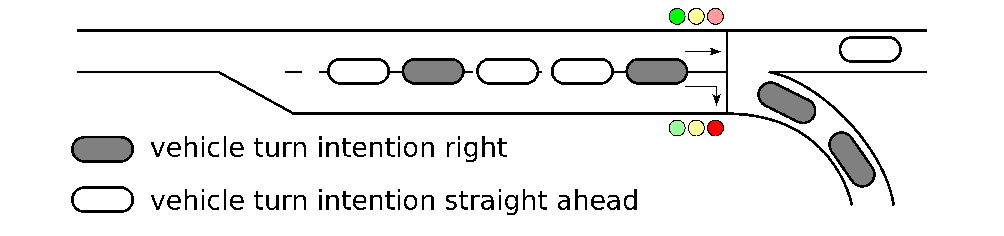
\includegraphics[width=0.5\textwidth, angle=0]{extending/figures/signalslanes/single_queue_model_inkscape.pdf} \end{center}

\editdone{This text has undergone the professional edit. Please no grammatical changes anymore! They are most-probably wrong.}
\createStandardInformationBasic{\url{http://matsim.org/javadoc} $\to$ core $\to$ signals}{The module is invoked by setting \lstinline|useSignalSystems| to \lstinline|true| in the config module \lstinline|scenario| }{Parameters are set in the config module \lstinline|signalsystems|.}{\citet{GretherBischoffNagel2011CottbusSylviaEventAbstract,Grether2014PhD}}

% ##################################################################################################################
\section{Motivation}
Traffic signals ensure security of travelers at junctions and regulate right of way. 
Furthermore, by assigning green times to the different approaches of a junction, they determine and evaluate junctions' performance. 
There are different strategies for traffic signal control: fixed-time traffic signal control, for example, periodically repeats the same schedule for signalization, while traffic-responsive signal control reacts dynamically to the prevailing traffic patterns, improving the junction or system performance overall.   
Even if traffic control improves the traffic conditions at a single junction, it might not benefit the whole system. 
\citet{Hu1997D2DFlowEvolutionReactiveSignalsDynasmart} argue that second order or network effects should be taken into account when effects of signal control strategies are tested. Network effects include drivers' reactions: not only route choice, but also scheduling. 
Thus, traffic control, especially traffic-responsive signals, need certain constraints. Otherwise, traffic may become unstable: rapidly at two nearby junctions, or at the network level \citep{LaemmerHelbing2010SelfStabilizingSignalControlRealNet}. \gls{matsim} can capture most of these effects. This chapter reviews concepts, usage and restrictions of the traffic signal control extension for \gls{matsim}. 
The chapter is particularly interesting for\gls{matsim} users, who plan to simulate traffic signals microscopically. 
If one wishes to capture signalization effects on a rather coarse level, consider the approach presented in~\citet[pp.~139][]{Charypar2008PhD}, that can be realized with the time variant network feature of \gls{matsim} \citep{00LaemmelGretherNagel2009TimeDependentNetworks}. 
Before we go into detail on motivating traffic signals with \gls{matsim}, a case study is reviewed. 

% ========================================================================================
\subsection{Case Study}
The Cottbus scenario presented in Chapter~\ref{ch:cottbus} is applied to illustrate the influence of traffic signal control. 
This section summarizes results published in~\citet{GretherBischoffNagel2011CottbusSylviaEventAbstract,Grether2014PhD}. Readers interested in details are referred to these publications. 

The runs sequence is performed with three different signal control strategies:
in a first simulation sequence, all traffic signals are switched off. This can be used as a lower bound for results of signal control, since it assumes that vehicles are able to traverse a crossing without an accident, \ie they are able to drive ``through each other''. 
The next sequence uses the fixed-time setup. 
In the third and final, sequence, all traffic signals are controlled by a traffic-actuated stage length control. 
The control is based on pre-timed, fixed-time schedules. 
The green times of the fixed-time schedules are reduced to a minimal green time of 5/10\,seconds. 
If vehicles are still approaching at the end of this reduced green time, it is extended up to a predefined maximum. 
%
\createfigure%
{Simulation results}%
{Simulation results for the Cottbus traffic signal scenario: The simulated change of traffic signal control results in small travel pattern changes in the relatively quiet commuter scenario (left). If unexpected traffic occurs on the network, the traffic-actuated signal control enables travel time savings (right).}%
{\label{fig:results_histogram}}
{%
  \createsubfigure%
  {No vs.~fixed-time vs.~traffic-actuated signal control, commuter traffic, iteration~1\,000}%
	{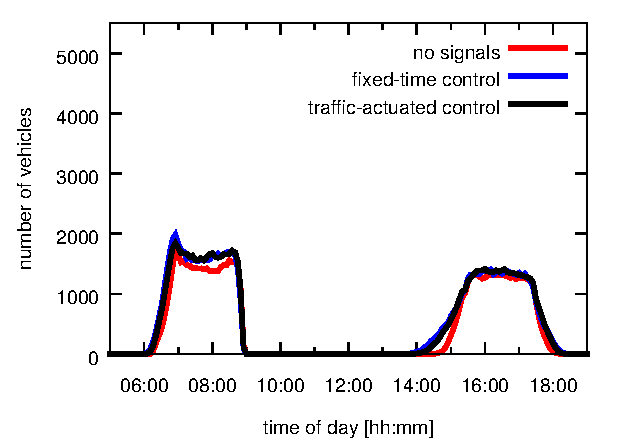
\includegraphics[width=0.48\linewidth]{extending/figures/signalslanes/leg_histogram_cottbus_1292_1293_1291_it_1000_book.pdf}}
  {\label{fig:commuter_traffic}}%
  \createsubfigure%
	{Average travel time for unexpected event traffic, iteration~1\,000}
	{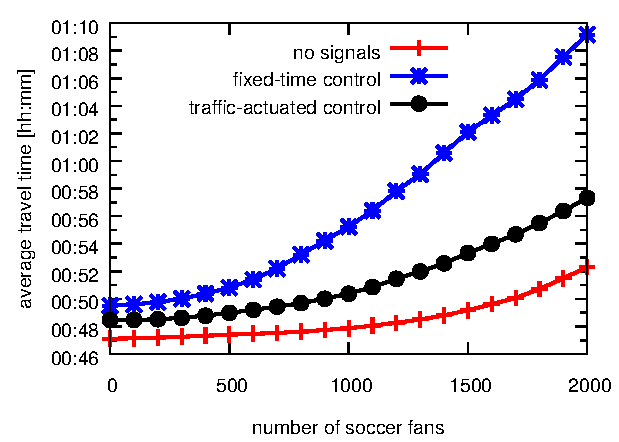
\includegraphics[width=0.48\linewidth]{extending/figures/signalslanes/average_travel_time_1220_1222_book.pdf}}
	{\label{fig:unexpected_event}}
}%
{\citet{Grether2014PhD}}

Simulation results for iteration~1\,000 of the Cottbus commuter scenario are depicted in Figure~\ref{fig:commuter_traffic}. The number of vehicles simultaneously on the road is plotted over the time-of-day. The results are quite similar for all signal control strategies; differences are small because of the lack of heavy congestion in the Cottbus scenario. 

A change of signal control has more effect if unexpected traffic occurs in the network. It is assumed that the local soccer club, ``FC Energie Cottbus'', has a tournament taking place on a normal weekday, interfering with regular commuter traffic. In iteration~1\,000 of the commuter scenario, in addition to the commuters 0 to 2\,000\,vehicles drive to the Cottbus soccer stadium during the evening peak. It is assumed that 25\,\% of these fans come from Cottbus, while the other 75\,\% come from the ``Spree-Nei{\ss}e'' area around Cottbus, and that all fans start their trips between 5\,pm and 6\,pm. 

Figure~\ref{fig:unexpected_event} plots the number of soccer fans on the x-axis, and the average travel time of all travelers on the y-axis. Without any additional vehicles, the traffic-actuated signal control leads to a gain of approximately 1\,minute per traveler. The more additional traffic approaches the stadium, the more the traffic-actuated control saves travel time. When 2\,000\,additional vehicles are on the road, travel time savings reach approximately 15\,minutes per traveler. 

Summarizing: Slightly jammed commuter scenarios, where a change in traffic signal control leads to noticeably decreased overall travel time, have not yet been simulated with \gls{matsim}. Looking at different objectives with more fine-grained analysis tools can reveal network wide effects~\citep[\eg see the analysis using macroscopic fundamental diagrams][pp.114]{Grether2014PhD}, but this is work in progress. More heavily jammed scenarios can increase the overall traffic impact of a change in traffic signal control. Nevertheless, the case study shows significant effects of traffic-responsive signal control when something unexpected happens and travelers do not react.  

% ========================================================================================
\subsection{Overview MATSim \& Traffic Signals}
This case study highlights some previously researched \gls{matsim} traffic signals simulations aspects. 
\gls{matsim} is not always the traffic signal control ``tool of choice'' for all questions. 
The code base, however, can help simulate other use cases, \eg evacuation or air transport scenarios; 
\gls{matsim}'s open source nature provides hooks and interfaces for extension. 
But one must consider the amount of work required, the current state of development and specific project planning. 
The rest of the chapter goes into more detail.  
Section~\ref{sec:signals_traffic_signal_control} provides some traffic signal control background, vocabulary and options for modeling traffic signals with \gls{matsim}. 
Technical details can be found in the traffic signals user guide.  
Section~\ref{sec:signals_network_traffic_flow} goes into details on network and traffic flow modeling. 
Iterations and learning are discussed in Section~\ref{sec:signals_iterations_learning}. 
When it comes to agent based learning, \gls{matsim} is very fast---the presented case study requires, on average, 17\,seconds computation time per iteration---for scoring, replanning, and output. One complete run sequence: (1\,000\,iterations, single core mobility simulation, multi-core replanning) was simulated in 9\,hours and 12\,minutes. 
The simulation speed allows exploration of network-wide behavioral reactions to  traffic signal control changes and 
the resource efficient simulation enables the joint simulation of several policies. 
Before publishing results, one should consider several specific aspects of evaluation and simulation results interpretation. 
Hints are provided in the conclusion,  Section~\ref{sec:signals_evaluation_conclusion}. 

% ##################################################################################################################
\section{Traffic Signal Control}
\label{sec:signals_traffic_signal_control}
On a coarse level, control strategies for traffic signals can be classified in fixed-time and traffic-responsive strategies. 

Fixed-time traffic signal control periodically assigns green times for each junction approach. 
Cycle time and green split are not modified within short time periods. 
To establish green waves between adjacent junctions, the green light start for approaches within the cycle can be adjusted by a global timer; 
these shifts are referred to as coordination offsets. 
For optimization of fixed-time signals, different equilibrium traffic flow regimes are determined for several periods of time, \eg weekday morning, midday, evening and night plus a separate estimate for weekends. Optimization may target all signalized junction parameters---green split, cycle, offsets, and phase composition,  
but it is not possible to react to current changes in equilibrium traffic flows. 

Traffic-responsive control reacts to current traffic patterns, adjusting traffic signal control parameters on the fly. 
In principle, all available information on prevailing traffic patterns can be used. 
The diversity of traffic-responsive control algorithms is wide; for a review, see~\citet[][]{Grether2014PhD}. 

\gls{matsim}'s traffic signal module is designed to simulate every traffic signal control strategy. 
The module provides a default implementation for fixed-time control. 
Traffic-responsive strategies require custom implementation of the control algorithm, but can use existing data formats and fixed-time control infrastructure. 
Data is divided into five different types of input:
%
\begin{description}\styleDescription
	\item[Signals \& Systems:] The location of the traffic signal hardware on the network is usually independent from the control strategy. 
		Signals can be located at the end of a link or a lane (see the next section for further discussion of lanes). Signals are attached to a system that reflects, \eg all signals of a junction or even larger units. 
		Each signal system is controlled by exactly one control algorithm at a time.  
	\item[Signal Groups:] Traffic signals must be attached to a group. 
		A group of signals shows the same color at the same time. 
		Each time a signal group changes its state, a \gls{matsim} event is triggered. 
		There is no explicit phase representation; 
		if required, this can be realized over signal groups.  
	\item[Signal Control:] Specifies the control algorithm for each signal system. 
		Data comprises information for fixed-time control and can be extended to capture custom control algorithms' parameters . 
	\item[Amber:] Specifies the amber phase at the beginning and end of green time. 
		Currently, this information is used only for visualization purposes. 
		Driving is not permitted if a traffic signal group shows amber light. 
	\item[Intergreens:] The inter-green time specifies minimal time period between the ending of one and beginning of another signal group's green time.  
		This information is important because \gls{matsim}'s traffic flow model does not contain any collision detection. 
		A validation module reads the event stream and triggers a warning, or an error, if security constraints are violated. 
		Further, customized control strategies can access this information to ensure security aspects' control validity.    
\end{description}

For detailed information on file structures and how to link them in the \gls{matsim} \gls{configfile}, we refer to the user guide in the contribution ``signals'', which we update periodically.

The next section explains network representation and traffic signal location in more detail. 

% ##################################################################################################################
\section{Network Representation \& Traffic Flow}
\label{sec:signals_network_traffic_flow}

\createfigure%
{Transition from a real road segment to a graph layout with a single queue}%
{Transition from a real road segment to a graph layout with a single queue: the missing turn pockets representation prevents vehicles passing each other and cannot capture the traffic signal control for different turning moves. }
{\label{fig:combined_model}}
{%
  \createsubfigure%
	{Typical real road layout}
	{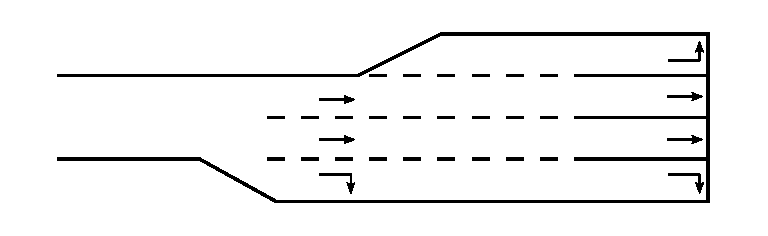
\includegraphics[width=0.475\linewidth]{extending/figures/signalslanes/real_road_layout.pdf}}
	{\label{fig:real_road_layout}}
  \createsubfigure%
	{Single queue, spill-back is not captured correctly}%
	{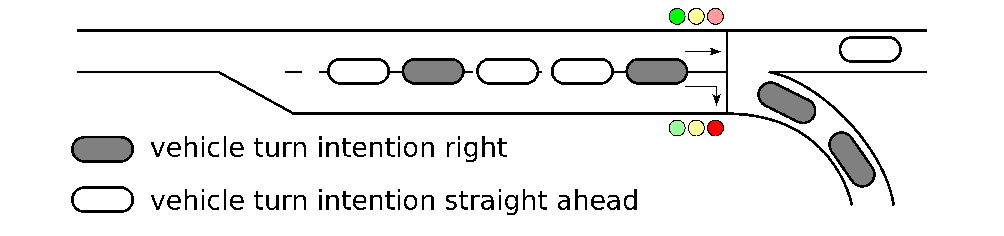
\includegraphics[width=0.48\textwidth]{extending/figures/signalslanes/single_queue_model_inkscape.pdf}}%
	{\label{fig:lanes_representation_single_queue}}%
}%
{\citet{GretherNeumannNagel2012SignalsQueueModelABMTrans}}

This section explains transport network representation with microscopically modeled traffic signals. 
In \gls{matsim}, transport network representation is a static, directed graph, consisting of nodes and links. 
Links depict road segments, while nodes can be interpreted as decision points in space with a coordinate as attribute, but no spatial dimension. 

Figure~\ref{fig:real_road_layout} illustrates a typical layout of a real-world road segment, with several turn pockets at its end. 
If the whole road segment is modeled as a single link with \gls{matsim}'s queue model, the first vehicle stopping at a red traffic signal at the end of this link will block all other vehicles approaching upstream, see Figure~\ref{fig:lanes_representation_single_queue}. 
In respect to the road layout shown in Figure~\ref{fig:real_road_layout}, this is unrealistic. 
Figure~\ref{fig:model_link_layout} sketches the network layout for a more realistic modeling. 
Vehicles with distinct turn intentions do not block each other until the available space for queuing on the turn pocket is used completely, see Figure~\ref{fig:lanes_representation_multiple_queue}. 

\createfigure%
{Transition from a real road segment to a graph layout with multiple queues}%
{Transition from a real road segment to a graph layout with multiple queues: each turn pocket is represented by its own queue. Traffic signal control for different turning moves is captured; vehicles can pass each other, unless the queue spills over. }
{\label{fig:lanes_representation}}%
{%
  \createsubfigure%
	{Part of the graph required to model the road layout}
	{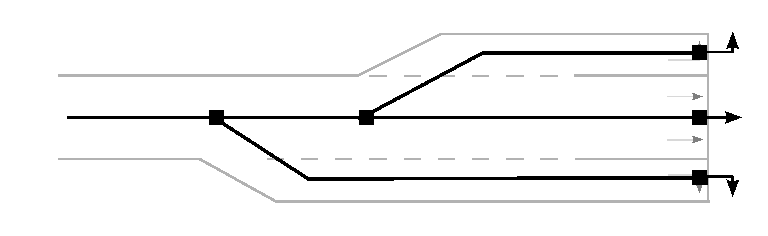
\includegraphics[width=0.475\textwidth]{extending/figures/signalslanes/link_lanes_layout}}
	{\label{fig:model_link_layout}}
  \createsubfigure%
	{Multiple queues, spill-back is captured correctly}%
	{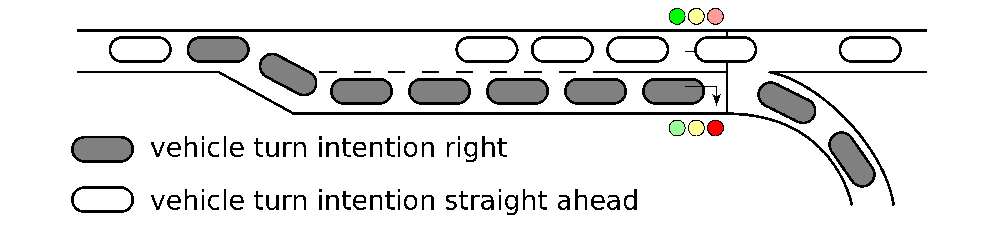
\includegraphics[width=0.48\textwidth]{extending/figures/signalslanes/multiple_queue_model_inkscape.pdf}}%
	{\label{fig:lanes_representation_multiple_queue}}%
}%
{\citet{GretherNeumannNagel2012SignalsQueueModelABMTrans}}

In principle, one can model each turn pocket as a link and put traffic signals at its end; 
but considering overall project constraints, this has implications for network modeling and routing. 

In \gls{matsim}, all domain-relevant attributes differing from geospatial location, \eg traffic count data, transit stops, transit lines, or speed limits, are attached to links. 
If one of this attributes changes, one must model several links. 
Frequently, geospatial location of such attributes is insufficient for a fully automatic matching of attributes to links; 
some data requires manual post-processing. 
To simulate traffic signals and turn pockets with an already existing scenario, carefully consider the matching process before changing the network.  

Travelers' routes are specified by link sequences within \gls{matsim} and 
routes are generated by a shortest path algorithm requiring a cost function for links. 
In standard \gls{matsim}, link travel time is part of a link's cost.
When modeling turn pockets as links, the shortest path algorithm is responsible for selecting the appropriate turn pocket on a route.
If modeling includes turn restrictions, ensure that they are captured by the shortest path algorithm and note that 
the required number of iterations increases if many turn pockets lead to the same downstream link. 
It is important to understand route generation and network modeling interaction when modeling turn pockets as links. 

If network modeling or routing issues clash with other project goals, there is an alternative. 
\gls{matsim} allows the modeling of a subgraph on top of each link to reflect the structure shown in Figure~\ref{fig:model_link_layout}. 
The links of the subgraph are then called \emph{lanes}. 
At the beginning of a link, only one lane can be modeled; at the end of a link, different lanes can exist to model turn pockets. 
A vehicle must  be in the correct turning lane for the next downstream link of its route. 
If there is only one lane towards the downstream link, the vehicle uses this lane. 
If there is more than one lane leading to the next downstream link, the vehicle is placed on the lane currently containing the fewest other vehicles.
Using lanes, specific turning moves can be forbidden because the shortest path algorithm underlying network graph is modified;  
thus, turn restrictions are considered when the network graph is created.  
The shortest path calculation captures the effects of lanes without further modification \citep[see][pp.~21]{Grether2014PhD}.  

As well the differences mentioned above, lanes exhibit behavior similar or equal to links.  
Vehicles entering or leaving lanes trigger events with the same structure and information as link enter and leave events.
Traffic signals can be placed at the end of links and lanes. 
Traffic on each lane is simulated the same way as for links. 
Traffic flow increase is linear in a signal's green time for both links and lanes. 

The decision to use or not use lanes is arbitrary. 
Most \gls{matsim} scenarios with signals are set up using lanes; the code base is well debugged. 
Without lanes, the code for traffic signals is also tested; one should check carefully for artifacts and understand influences on route generation. 

% ##################################################################################################################
\section{Iterations \& Learning}
\label{sec:signals_iterations_learning}
This section discusses interaction between traffic signals and travelers within the \gls{matsim} iteration cycle. 

\citet{Meneguzzer1997ModelReviewTrafficAssignmentSignalControl} defines the combined traffic assignment and control problem as finding a tuple $(f^{*}, g^{*})$ of traffic flows $f$ and signal settings $g$ under policy $P$ that fulfills  
\[
f^{*} = f^{e}[g^{P}(f^{*})] \mbox{  or  equivalently } g^{*} = g^{P}[f^{e}(g^{*})]
\]
where $f^{e}$ is a function mapping signal settings to equilibrium traffic flows and $g^{P}$ a function mapping traffic flows to signal settings under policy $P$.  
The formulation neatly shows the mutual interaction of traffic patterns and signal settings.  
The formulations do not capture the time horizon where these interactions take place. 

Traffic signal interpretation within the \gls{matsim} iteration cycle depends strongly on signal control type and learning mechanism interpretation. 
For fixed-time control, the fixed-point interpretation can be valid, at least if one does not anticipate  unexpected events on the demand side. 
For traffic-actuated signal control strategies, no standard interpretation can be provided. 
Readers seeking more detail are referred to~\citet[][pp.~75]{Grether2014PhD}.  
We conclude with this advice; clearly document what and how was simulated and provide an interpretation that makes sense for each individual project.    

% ##################################################################################################################
\section{Conclusion} 
\label{sec:signals_evaluation_conclusion}
\gls{matsim} can simulate traffic signal control microscopically. 
However, certain traffic signal effects are not represented by \gls{matsim} without further customization and implementation, \eg microscopic deceleration and acceleration as a reaction to traffic control. Evaluations must be checked and interpreted against the simulation setup to ensure that everything derived from simulation results is also appropriately simulated.  
This chapter provides an overview of traffic signals in \gls{matsim}, detailing what to consider before taking first steps in larger scenarios. Further details can be found in the \gls{javadoc} documentation referenced above. 

We think that \gls{matsim} is a superior tool for microscopic simulated traffic-responsive signal control that should be analyzed network-wide, assuming heterogeneous user reactions. 

%As technical documentation quickly becomes outdated, the chapter tries to avoid technical detail; as there is also an incrementally improving user guide\footnote{Find the user guide  in the contribution "signals" where in future days the package \lstinline|signalsystems| is moved \kai{vermutl.\ \url{http://ci.matsim.org:8080/job/MATSim_contrib_M2/org.matsim.contrib$signals/javadoc/?}, sobald es functioniert.}}. 
 
% ##################################################################################################################
%\section{Automatically Generated Module Information}
%\label{sec:signals_config}
%Module in the config: 
%\begin{itemize}
%	\item \lstinline|signalsystems|
%\end{itemize}
%
%Package:
%\begin{itemize}
%	\item \lstinline|org.matsim.signalsystems|
%\end{itemize}
%
%http://matsim.org/node/732
%
%Literature: \citet[][]{GretherEtAl_ABMTRANS_2012, Grether_PhDThesis_2014, Neumann_MastersThesis_2008}
%Auch Miss Ou-Paper ansehen: Optimierung von Lichtsignalen
%
%Information about signal light timing is available for the city of Zurich  \citep{STAPOZH-DAV_unpub_gtZH_2008} (\ref{ptl:zhCity}). Modeling of traffic lights was implemented for the project \emph{Westumfahrung} through reducing the available link capacity. However, the used \emph{mobsim} (DEQSim) is deprecated (see Section \ref{sec:deqsim}).
%
%Research and implementation efforts are undertaken to include individual traffic lights in other \emph{mobsims} (see e.g., (\ref{tl:docu}) and \citet[][]{Neumann_MastersThesis_2008}).
%
%% -------------------------------------------
%
%Lanes:
%
%The lanes package has been implemented in conjunction with signal systems. Lanes are enabled in the \lstinline|scenario| configuration file section. The lanes package (\lstinline| org.matsim.lanes|) provides readers, where the class \lstinline|ModelLane| serves as the interface between the lane functionality and the mobility simulation. The lane definitions file needs to be specified in the \lstinline|network| configuration file section.

% ##################################################################################################################
